\chapter{Verwendete Methodiken}
Nach der Einführung zu den verschieden Themenbereichen, nur zu den eigentlichen Methodiken, welche entweder schon vorhanden sind, oder im Zuge dieser Arbeit erarbeitet wurden.
\section{Verfügbare Daten}
\label{cap:background_sec:setting}
Nun wird die Herkunft der für die nächsten Kapitel elementaren Daten erläutert. Ein Elektrofahrzeug verfügt über folgende Daten, die Ankunftszeit an der Ladestation für den aktuellen Ladezyklus, die Abfahrtszeit, wenn diese erreicht ist endet der aktuelle Ladezyklus. Ebenso gibt jedes Fahrzeug für sich an, ob es gerade verfügbar ist, sprich mit einer Ladestation verbunden ist, welchen Ladezustand der im Fahrzeug verbaute Akku aktuell hat, sowie die aktuell mögliche Ladeleistung. Die Ladegräte wissen jeweils welche Leistung sie gerade an das mit ihnen verbunden Elektrofahrzeug abgeben, sofern den ein Elektrofahrzeug mit ihnen verbunden ist. Einige Daten sind auch aus dem Stromnetz an sich bekannt, so ist die Leistungsabgabe des Transformators ans Stromnetz bekannt, sowie für jeden betrachten Hausanschluss, das dort aktuell vorherrschende Spannungslevel.

\section{Spannungsregler nach VDE 4100}
\label{capBody:VDE}
Die erste Methodik dient als Grundlinie für den Vergleich der später folgenden Methodiken. Diese Methodik stellt die aktuell im Stromnetz vorliegende Situation dar. Sie verwendet die technische Anschlussregel Niederspannung (VDE-AR-N 4100), diese stellt neue Anforderungen an die Ladegeräte von Elektrofahrzeugen. Sie wurde ebenfalls entwickelt, um eine größere Anzahl von Ladegeräten am Netz nutzbar zu machen (VDE-quelle). Bei der verwendeten Form der Anschlussregel, handelt es sich um einen Spannungsregulator, welcher anhand der Spannung angibt, wie viel der aktuell möglichen Leistung abgerufen wird. Bei einem gemessenen Wert der Spannung von mehr als 93\% der Normspannung, kann die Leistung wie gefordert abgerufen werden. Ab einer Spannung von weniger als 88\% der Normspannung kann keine Leistung mehr angerufen werden. In dem Bereich von 93\% bis 88\% der Normspannung wird die abrufbare Leistung linear reduziert, von voller hin zu keiner abrufbaren Leistung.

\begin{figure}[htb]
	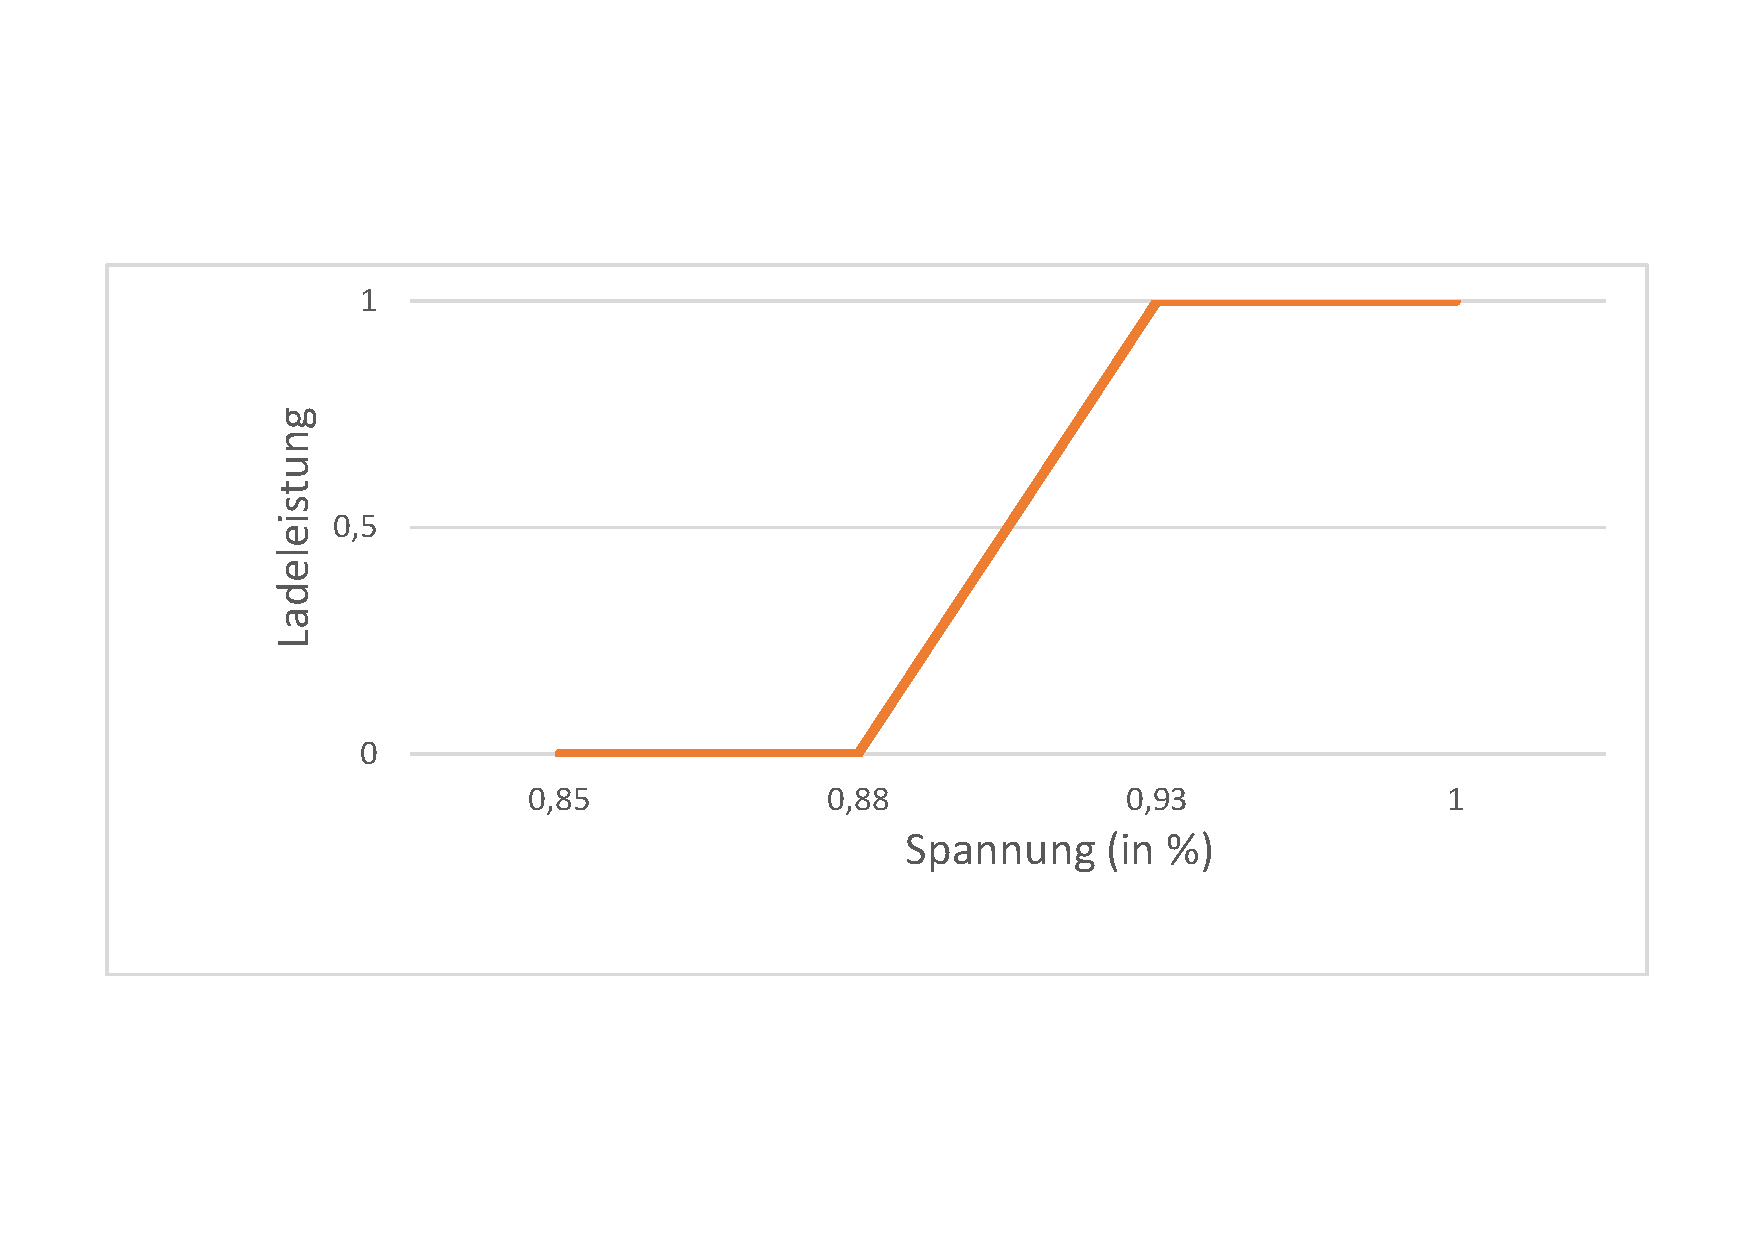
\includegraphics[width=\linewidth]{img/Dia2.pdf}
	\caption{Spannungs zu Leistungsverhältnis nach VDE-AR-N 4100(grün)}
	\label{Abb_VDEController}
\end{figure}

Der Graph in Abbildung \ref{Abb_VDEController} zeigt die mögliche Ladeleistung bei dem prozentualen Anteil der Normspannung. Auf der Y-Achse ist die mögliche Ladeleistung angetragen, wobei die eins für die höchstmögliche Leistung steht und null dafür, dass für keine Leistung abrufbar ist. An der X-Achse werden die aktuell anliegenden Prozent der Normspannung angetragen. An dem Graphen ist ersichtlich, dass bei mehr als 93\% der Normspannung die ganze Ladeleistung zur Verfügung steht. Es ist weiterhin erkennbar, wie sich die mögliche Ladeleistung im Bereich von 93\% bis 88\% der Normspannung verhält. Ebenso, wie das keine Ladeleistung bei einem Wert von weniger als 88\% der Normspannung mehr möglich ist. \\
Die Ladeleistung wird berechnet durch die Formel
\begin{align}
	Ladeleistung = Aktuelle\ Spannung \cdot maximal \label{Main_formula1}\\
	nutzbare\ Stromst\ddot{a}rke\ des\ Fahrzeuges \nonumber
\end{align}
Bei der Formel \ref{Main_formula1} wird von einer Spannung von über 93\% der Normspannung ausgegangen, da die berechnete Ladeleistung nicht verändert wird. Im Bereich von 93\% bis 88\% der Normspannung ist eine solche Änderung aber nötig. Der Faktor F, mit dem der verbliebene Anteil der möglichen Ladeleistung bestimmt wird, wird mit der Formel \\
\begin{align}
	F = 20 \cdot \frac{aktuelle Spannung}{Normspannung} - 17.6
	\label{Main_formula2}
\end{align}
Berechnet. Der Wertebereich der Formel ist bei null bzw. Eins abgeschlossen. Bei zu niedrigen Spannungswerten, weniger als 88\% der Normspannung, wird der Faktor ohne Berechnung der Formel mit null angegeben. Ergebnisse größer als eins werden auf eins reduziert, da alle Werte größer als eins in einer höheren Ladeleistung als überhaupt möglich resultieren würden. Wird nun der Faktor in Formel \ref{Main_formula1} berücksichtigt, ergibt sich folgende Formel für die mögliche Ladeleistung
\begin{align}
	Ladeleistung = Aktuelle\ Spannung \cdot maximal\ \label{Main_formula3}\\
	nutzbare\ Stromst\ddot{a}rke des\ Fahrzeuges \cdot Faktor \nonumber
\end{align}
Bevor die berechnete mögliche Ladeleistung allerdings tatsächlich bezogen wird, wird der Wert mithilfe eines First-Order Lag Filters gefiltert. Bei einem First-Order Lag Filter wird eine Änderung zwischen dem aktuellen und einem neu berechneten Wert nicht komplett vollzogen, sondern nur teilweise. Ein solcher Filter dient der Dämpfung großer Änderungen und soll kleiner Änderungen fast unverändert lassen. In der hier verwendeten Form werden nur 63,2\% der eigentlichen Änderung vorgenommen. So steigen Werte nur um 63,2\% der eigentlichen Steigerung, ebenso fallen Werte nur um 63,2\% der Änderung.
\begin{figure}[htb]
	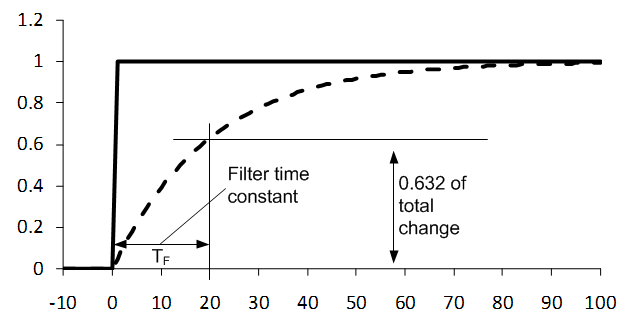
\includegraphics[scale=0.75]{img/lag_Filter.png}
	\caption{Spannungs zu Leistungsverhältnis nach VDE-AR-N 4100(grün)}
	\label{Abb_lag_filter}
\end{figure}

Aus der Abbildung \ref{Abb_lag_filter} wird ersichtlich, wie ein First-Order lag Filter auf ein starkes Wachstum eines Wertes reagiert. Die fett markiert, durchgezogene Linie zeigt den Verlauf ohne Filter. Die fett markierte, gestrichelte Linie zeigt den Verlauf mit Filter. T\textsubscript{F} zeigt die Dauer des verwendeten Zeitintervalls. Die zwei dünnen, schwarzen Linien markieren an ihrem Schnittpunkt den Wert nach der ersten Anwendung des Filters. Dieser Wert liegt bei 63,2\% der eigentlichen Änderung. Bei fortlaufender Zeit nähert sich die fett markierte, gestrichelte Line der fett markierten, durchgezogen Linie immer weiter an.

\section{Verbesserte Spannungsregler}
Bei den nächsten vorgestellten Methoden wurden Bestandteile des Slotted Aloha Protokolls (Kapitel \ref{capBack:Aloha}) verwendet. Das Slotted Aloha Protokoll arbeitet auf einem geteilten Medium, welches von allen Teilnehmern verwendet wird. Dieses geteilte Medium ist in diesem Fall das in Kapitel \ref{capBack:Stromnetz} vorgestellte Niederspannungsnetz mit den dazugehörigen elektrischen Leitern. Ein Frame des Aloha Protokolls entspricht der Leistung die für die einzelnen Teilnehmer über das Stromnetz verteilt wird. Eine Kollision tritt immer dann auf, wenn die Spannung bei einem einzelnen Teilnehmer zu niedrig wird oder die Last am Transformator des Netzes zu hoch wird. Ob und wie nun auf die verschiedenen Arten der Kollisionen reagiert wird, hängt von der verwendeten Methodik ab.
\subsection{Wartezeit über Teilnehmerzahl}
\label{cap:background_sec:SA_participants}
Der in Kapitel \ref{capBody:VDE} vorgestellte Spannungsregler wird um die Behandlung von lokalen Spannungskollisionen, welche bei jedem Teilnehmer individuell passieren können, erweitert. Eine Spannungskollision tritt immer dann auf, wenn der Wert der lokal gemessen Spannung auf unter 88\% der Normspannung fällt. Fällt die Spannung auf einen solch niedrigen Wert kann gemäß dem Spannungsregler keine Leistung mehr aus dem Netz bezogen werden, bis die Spannung wieder auf einen Wert von über 88\% der Normspannung steigt. Ist eine Spannungskollision aufgetreten, wird, geregelt durch den Spannungsregler, keine Leistung mehr aus dem Netz bezogen und eine Wartezeit bestimmt. Diese Wartezeit gibt an, wie lange der Teilnehmer nicht mehr versucht Leistung aus dem Netz zu beziehen. Diese Wartezeit wird auch eingehalten, wenn die gemessen Spannungswerte eigentlich wieder einen Leistungsbezug möglich machen würden. Der Wert der Wartezeit werden per Zufall aus einem Intervall heraus bestimmt, unter Verwendung eines Mersenne-Twister(python-random). Das Intervall ist nach unten sowie oben begrenzt. Die untere Grenze ist die Null, was keiner Wartezeit entspricht. Die obere Grenze wird primär durch die aktuelle Anzahl an Teilnehmer bestimmt. Jedes Fahrzeug, welches aktuell mit dem Stromnetz verbunden ist und dessen Ladezustand unter 100\% liegt, gilt in diesem Fall als Teilnehmer. Diese Abgrenzung wurde getroffen, da auch nur diese Teilnehmer, welche in diese Gruppe fallen, auch Leistung aus dem Netz beziehen können. Die Anzahl der Teilnehmer kann nicht von einem Teilnehmer selbst bestimmt werden. Eine zentrale Stelle ermittelt, welche der möglichen Teilnehmer, mit einem Ladegerät verbunden sind und einen Ladezustand von unter 100\% aufweisen. Diese zentral bestimmte Anzahl wird dann an alle diese Teilnehmer verteilt. Ein Sonderfall tritt ein, wenn die Menge der Teilnehmer zahlenmäßig höher ist als die Anzahl der Zeiteinheiten zwischen dem aktuellen Zeitpunkt und dem Zeitpunkt an dem das Fahrzeug die Ladestation wieder verlässt. Wenn dieser Fall eintritt, wird das Intervall, aus welchem die Zufallszahl heraus bestimmt wird, nicht von der Anzahl der Teilnehmer nach oben hin begrenzt. Die obere Grenze des Intervalls entspricht dann der Anzahl von Zeiteinheiten zwischen dem aktuellen Zeitpunkt und dem Zeitpunkt an dem das Fahrzeug die Ladestation wieder verlässt. Es besteht die Möglichkeit, dass wenn die Wartezeit abgelaufen ist wieder oder immer noch eine Spannungskollision vorliegt. Tritt dies ein, wird wieder eine Wartezeit bestimmt, es gibt keine Möglichkeit für eine Sonderbehandlung bzw eine minimale Ladezeit nach einer Wartezeit. Diese hier vorgestellte Methodik wurde nur um Funktionalität für Spannungskollisionen erweitert. Wenn eine zu hohe Last vom Transformator abgerufen wird, werden bei dieser Methodik allerdings keine Maßnahmen ergriffen.
\begin{figure}[htb]
	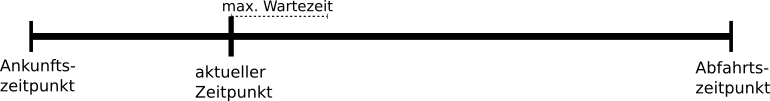
\includegraphics[width = \linewidth]{img/SA_participants_Graph2.png}
	\caption{Graph}
	\label{SAPart:Graph}
\end{figure}

\subsection{Wartezeit über Teilnehmer und Fahrzeugparameter}
Der in Kapitel .. vorgestellte Spannungsregler wird um die Behandlung von lokalen Spannungskollisionen, welche bei jedem Teilnehmer individuell passieren können, erweitert. Eine Spannungskollision tritt immer dann auf, wenn der Wert der lokal gemessen Spannung auf unter 88\% der Normspannung fällt. Fällt die Spannung auf einen solch niedrigen Wert kann gemäß dem Spannungsregler keine Leistung mehr aus dem Netz bezogen werden, bis die Spannung wieder auf einen Wert von über 88\% der Normspannung steigt. Ist eine Spannungskollision aufgetreten, wird, geregelt durch den Spannungsregler, keine Leistung mehr aus dem Netz bezogen und eine Wartezeit bestimmt. Diese Wartezeit gibt an, wie lange der Teilnehmer nicht mehr versucht Leistung aus dem Netz zu beziehen. Diese Wartezeit wird auch eingehalten, wenn die gemessenen Spannungswerte eigentlich wieder einen Leistungsbezug möglich machen würden. Der Wert der Wartezeit werden per Zufall aus einem Intervall heraus bestimmt, unter Verwendung eines Mersenne-Twister(python-random). Das Intervall ist nach unten sowie oben begrenzt. Die untere Grenze ist die Null, was keiner Wartezeit entspricht. Die obere Grenze wird durch Ausführung einer Formel bestimmt, welche von drei Parametern abhängt.  Der erste Parameter gibt an wie viele Zeiteinheiten, zwischen dem aktuellen Zeitpunkt und dem Zeitpunkt, an dem das Fahrzeug die Ladestation wieder verlässt, liegen. Dieser Parameter wird im Folgenden mit ‚verbleibender Zeit‘ bezeichnet. Der zweite Parameter gibt an, wie viel Zeit noch benötigt wird, um den Akku des Fahrzeuges auf einen Ladestand von 100\% zu bringen. Für diese Berechnung wird allerdings die Normspannung verwendet und nicht die aktuell gemessene Spannung. Dieser Parameter wird im Folgenden mit ‚verbleibender Ladezeit‘ bezeichnet. Die beiden Parameter, verbleibende Zeit und verbleibende Ladezeit, werden lokal von jedem Teilnehmer für sich selbst bestimmt, sie benötigen dafür keinen weiteren Input. Der dritte Parameter ist die aktuelle Anzahl an Teilnehmenden. Jedes Fahrzeug, welches aktuell mit dem Stromnetz verbunden ist und dessen Ladezustand unter 100\% liegt, gilt in diesem Fall als Teilnehmer. Diese Abgrenzung wurde getroffen, da auch nur diese Teilnehmer, welche in diese Gruppe fallen, auch Leistung aus dem Netz beziehen können. Die Anzahl der Teilnehmer kann nicht von einem Teilnehmer selbst bestimmt werden. Eine zentrale Stelle ermittelt, welche der möglichen Teilnehmer, mit einem Ladegerät verbunden sind und einen Ladezustand von unter 100\% aufweisen. Diese zentral bestimmte Anzahl wird dann an alle diese Teilnehmer verteilt. Diese drei Parameter, die verbleibende Zeit, die verbleibende Ladezeit und die Anzahl der Teilnehmer werden in folgende Formel eingesetzt:
\begin{align}
	obere \ Grenze = \frac{verbleibende\ Zeit - verbleibende\ Ladezeit}{Anzahl\ der\ Teilnehmer}
	\label{SA:formel4}
\end{align}
Das Ergebnis dieser Formel beschränkt nun das Intervall, aus dem die Wartezeit bestimmt wird, nach oben. Ein Sonderfall tritt auf, wenn das Ergebnis dieser Formel kleiner ist als eins. Dies kann passieren, wenn etwa die verbleibende Zeit geringer ist als die verbleibende Ladezeit. Tritt dieser Fall ein wird erneut eine obere Grenze für das Intervall bestimmt. Die Formel, die in diesem Fall verwendet wird, hat nur einen Parameter. Dieser Parameter ist die zuvor berechnete obere Grenze des Intervalls, genannt 'alte Grenze'. Zur Bestimmung des neuen Wertes wird folgende Formel verwendet
\begin{align}
	obere\ Grenze = 10 \cdot (1 - e^{alte\ Grenze - 1}) + 1
	\label{SA-formel5}
\end{align}
Das Ergebnis dieser Formel grenzt nun das Intervall, aus dem die Wartezeit bestimmt wird, nach oben ab. Das Verhalten während einer Wartezeit, welche mithilfe dieser Formel \ref{SA-formel5} abgegrenzt wurde, kann sich von dem Verhalten einer Wartezeit welche durch Formel \ref{SA:formel4} abgegrenzt wird unterscheiden. Wenn eine solche Wartezeit das erste Mal bestimmt wird, unterscheidet sich das Verhalten in drei Punkten. Der Erste wäre, dass die Verbindung zum Netz nicht getrennt wird, es wird also weiterhin Leistung aus dem Netz bezogen. Der zweite Unterschied liegt in der Bestimmung der möglichen Ladeleistung, statt mit der Formel \ref{Main_formula3} wird, entgegen dem eigentlich verwendetem Spannungsregler, die Formel \ref{Main_formula1} verwendet. Der dritte Unterschied ist das veränderte Verhalten beim Auftreten von Kollisionen, diese werden nicht beachtet und es wird nicht auf sie reagiert. Eine solche Art der Wartezeit kann allerdings nicht mehrmals direkt hintereinander wahrgenommen werden. Tritt nach Beendigung dieser Wartezeit sofort wieder eine Kollision auf, muss eine normale Wartezeit abgewartet werden, auch wenn das Intervall mithilfe der Formel \ref{SA-formel5} begrenzt wurde. Nach dieser Wartezeit ist eine solche Sonderbehandlung allerdings wieder möglich. Diese hier vorgestellte Methodik wurde nur um Funktionalität für Spannungskollisionen erweitert. Wenn eine zu hohe Last vom Transformator abgerufen wird, werden bei dieser Methodik allerdings keine Maßnahmen ergriffen.
\begin{figure}[htb]
	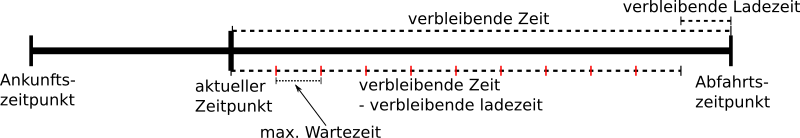
\includegraphics[width = \linewidth]{img/SA_waiting_Graph3.png}
	\caption{Graph}
	\label{SAWait:Graph}
\end{figure}
\begin{figure}[htb]
	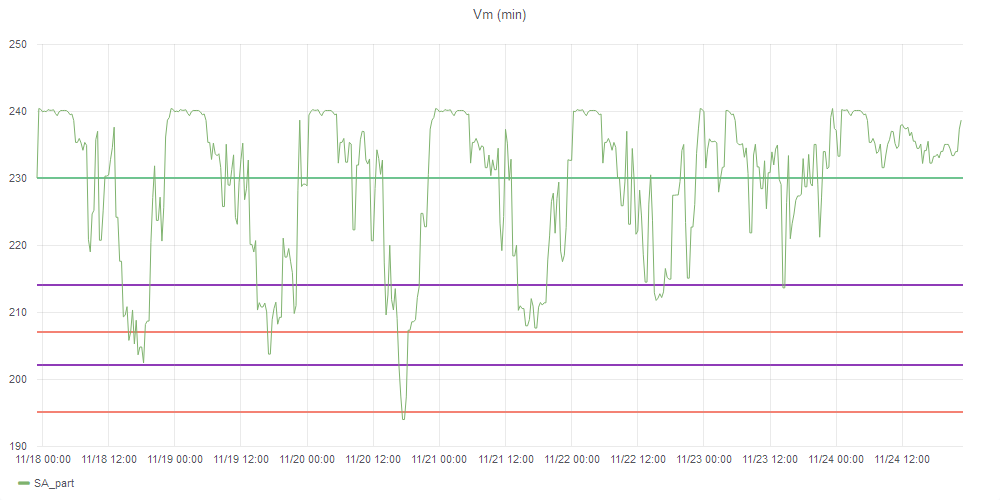
\includegraphics[width=\linewidth]{img/dia1.png}
	\caption{Diagram}
	\label{dia1}
\end{figure}

